\section{1. Comparaci\'on entre m\'etodos de medici\'on de puentes}

\subsection{Consideraciones generales}
Los puentes de medici\'on son configuraciones circuitales que permiten realizar mediciones a partir de la comparaci\'on de elementos cuando la combinaci\'on de estos
llevan a la condici\'on de equilibrio al puente. Se define tal condici\'on de equilibrio cuando la tensi\'on medida $V_d = 0V$ como se ilustra en la Fig. \ref{fig:puente_de_medicion}.

\begin{figure}[H]
    \centering
    \includegraphics[scale=0.5]{Recursos/puente.png}
    \caption{Circuito de un puente de medici\'on gen\'erico}
    \label{fig:puente_de_medicion}
\end{figure}

La aplicaci\'on pr\'actica de estos circuitos implica realizar un ajuste midiendo la salida diferencial del puente y observando en qu\'e situaci\'on se alcanza la condici\'on de equilibrio, es por ello
que es de gran inter\'es determinar los diferentes m\'etodos a emplear para poder medir de la mejor forma posible, cu\'Ando se alcanza el valor m\'inimo de $V_d$ asumiendo impedimentos que eviten alcanzar el valor nulo.

Los principales factores a tener en cuenta en el an\'alisis de los m\'etodos de medici\'on del puente son, en primer lugar, la capacidad de medir la salida diferencial del puente, teniendo en cuenta que toda se\~nal el\'ectrica
puede contar con la presencia de ruido, sea externo o interno del circuito, con lo cual el orden de magnitud de la variable de inter\'es se vuelve apreciable en t\'erminos del piso de ruido en diferentes escenarios.

\subsection{Osciloscopio}
El proceso de medici\'on en un osciloscopio consiste en utilizar dos canales para medir las tensiones referidas en la Fig. \ref{fig:puente_de_medicion} como $V_A$ y $V_B$, empleando luego la funcionalidad Math para obtener el resultado
de la resta de ambas, con lo cual efectivamente se podr\'ia medir la salida de inter\'es del puente, pudiendo observar as\'i su evoluci\'on en el tiempo, su amplitud y fase. La dificultad de este procesos es la capacidad de determinar cu\'ando la se\~nal que se mide,
en conjunto con el ruido, corresponde al equilibrio del puente.

\begin{figure}[H]
    \centering
        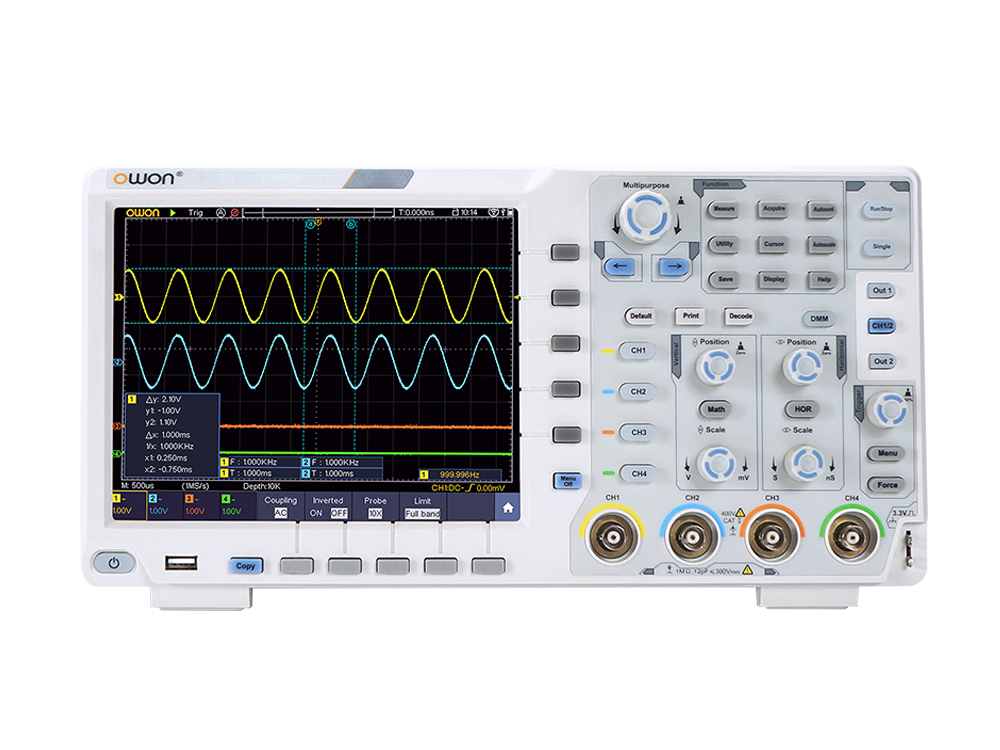
\includegraphics[scale=.8]{Recursos/oscilloscope.png}
    \caption{Osciloscopio Digital}
    \label{fig:osciloscopio}
\end{figure}

\subsection{Mult\'imetro de precisi\'on}
El mult\'imetro de precisi\'on permite realizar una medici\'on de una salida diferencial directamente, permitiendo realizar mediciones con mayor precisi\'on respecto del osciloscopio puesto que
no deben realizarse procesos adicionales sobre la medici\'on. Por otro lado, no se puede ver la se\~nal en el tiempo ni medir su fase, aunque en beneficio tiene menos error asociado al ruido.

\begin{figure}[H]
    \centering
        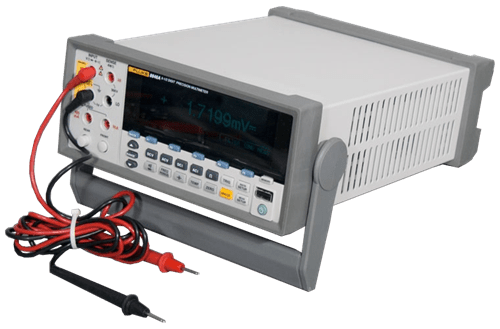
\includegraphics[scale=0.5]{Recursos/precision.png}
    \caption{Mult\'imetro de precisi\'on}
    \label{fig:multimetro}
\end{figure}

\subsection{Amplificador de instrumentaci\'on}
Un amplificador de instrumentaci\'on es un amplificador diferencial, esto es que amplifica una entrada diferencial, cuyas caracter\'isticas est\'an mejoradas en torno a la aplicaci\'on el mismo
en circuitos de se\~nales peque\~nas que pueden ser apreciables al ruido como salidas de transductores u otros tipos de sensores. Dentro de tales caracter\'isticas, se define la Relaci\'on de Rechazo de Modo Com\'un (CMRR) como la relaci\'on
entre lo que amplifica la entrada diferencial y aten\'ua la entrada en modo com\'un asociada al ruido. Es por dicha caracter\'istica que este tipo de circuitos puede ser muy apropiada para la calibraci\'on de un puente,
con lo cual la medici\'on resultante va a tener mucha mayor precisi\'on y puede emplearse un osciloscopio para visualizar tal resultado.

\begin{figure}[H]
    \centering
        
\includegraphics[scale=0.3]{Recursos/instrumentation.png}
    \caption{Esquema de un posible circuito de amplificador de instrumaci\'on}
    \label{fig:amplificador_instrumentacion}
\end{figure}